% Header: Here are all packages used and some additional definitions
%%%%%%%%%%%%%%%%%%%%%%%%%%%%%%%%%%%%%%%%%%%%%%%%%%%%%%%%%%%%%%%%%%%

\documentclass[11pt,a4paper]{scrartcl}
\usepackage[margin=2.5cm]{geometry}
\usepackage[onehalfspacing]{setspace}
\usepackage{graphicx} % zum Einbinden von Graphiken
\usepackage[breaklinks=true,colorlinks=true,linkcolor=blue,urlcolor=blue,citecolor=blue]{hyperref} % f. Referenzen
\usepackage{amsmath,amsthm,amssymb,amsfonts} % Mathematik Umgebung 
\usepackage{icomma} % Intelligentes Komma, das den richtigen Abstand zwischen Dezimalzahlen als auch in Formeln wählt.
\usepackage[ngerman]{babel} % Deutsche Bezeichnungen bei Inhaltsangabe etc
\usepackage[utf8]{inputenc}
\usepackage[T1]{fontenc}    % andere Schriftsatzkodierung für richtige Silbentrennung bei Umlauten
\usepackage{afterpage} % NEUE
\usepackage{hyperref}
\usepackage{cleveref}
\usepackage[locale = DE,space-before-unit=true,per-mode = symbol]{siunitx} % Bessere Einheiten
\usepackage{booktabs,multirow} % Pakete zur Erstellung von Tabellen
\usepackage{placeins} % Definiert den Befehl “\FloatBarrier”, der die Ausgabe der davor eingebundenen Bilder erzwingt, befor der Text weiter geht. (Mit vorsicht zu verwenden)
\usepackage[natbib,abbreviate=true,doi=false,style=numeric-comp,giveninits=true,sorting=none]{biblatex} % Modernes Paket zur Erzeugung von Bibliografien (benötigt biber!)
\usepackage{csquotes} % Fortgeschrittene Funktionen für Zitate, für die deutsche Form der Anführungszeichen bei Referenzen
\usepackage{minted} %für Code
\usepackage{listings}

\lstset{
  language=C++,
  literate=%
    {ä}{{\"a}}1
    {ö}{{\"o}}1
    {ü}{{\"u}}1
    {Ä}{{\"A}}1
    {Ö}{{\"O}}1
    {Ü}{{\"U}}1
    {ß}{{\ss}}1
}
\addbibresource{MyBibliography.bib} % Ort der .bib Datei, die die Datenbank für Literatur/Referenzen enthält.

\graphicspath{{Bilder/}}

\DeclareSIUnit{\dBm}{dBm}
\DeclareSIUnit[per-mode=reciprocal]\WN{\per\centi\meter}
%%%%%%%%%%%%%%%%%%%%%%%%%%%%%%%%%%%%%%%%%%%%%%%%%%%%%%%%%%%%%%%%%%%
\begin{document}
%
\titlehead{\includegraphics[width=5cm]{}} %Bild oben links 
\title{Proseminar: Effiziente Algorithmen}

\author{Name\thanks{\href{mailto:name@mail.de}{name@mail.de}} \\Universität}
\date{2. Februar 2024}
\maketitle
\vfill
Proseminarleiter: Name meines Professors
\newpage
\renewcommand\abstractname{Kurzfassung}
\section*{\abstractname}
Diese Arbeit präsentiert Lösungsansätze zu zwei ausgewählten Problemen des mehrstufigen Programmierwettbewerbs, International Collegiate Programming Contest (ICPC). Die Probleme entstammen den jeweiligen finalen Runden des Wettbewerbs. Das Problem "Gene Folding", aus dem Jahr 2020, bezieht sich auf das effiziente Finden von Palindromen. Das zweite Problem "\text{A Safe Bet}" \string erfordert eine effiziente Berechnung von Schnittpunkten horizontaler und vertikaler Geraden und stammt aus dem Jahr 2012.
\thispagestyle{empty}
%
%
\tableofcontents
\thispagestyle{empty}
\cleardoublepage
\pagenumbering{arabic} 
\newpage
%
%
\newpage
\section{Problem D: Gene Folding}
\label{sec:Latex}
\subsection{Beschreibung der Problemdomäne}
\label{subsec:DokHeadGli}
Es wird eine einzelne genetische Sequenz vorgegeben, welche ausschließlich aus den Zeichen “A”, “C”, “G” und “T” besteht.

Die Darstellung der genetischen Sequenz kann bis zu vier Millionen Zeichen enthalten. Dabei kann die Sequenz in ihren Zeichen reduziert werden. Falls eine Stelle \textit{s} innerhalb der Sequenz existiert, für welche gilt, dass, ausgehend von \textit{s},  die linke Teilsequenz und die rechte Teilsequenz identisch sind und zusätzlich die linke Teilsequenz bis zum Präfix oder die rechte Teilsequenz bis zum Suffix reicht, darf die Sequenz bis zur Stelle \textit{s} reduziert werden. Dabei wird die Teilsequenz, welche bis zu einem Ende der Sequenz reicht, ausgeschnitten. Das Ziel besteht darin, eine minimale Sequenz zu bilden und die Länge dieser Sequenz auszugeben.
%
\subsection{Erkenntnisse}
\label{subsec:TextBefehle}
Bei der Eingabe handelt es sich um eine Sequenz von Zeichen und folglich um eine Zeichenkette. Die gegebene Zeichenkette kann durch Palindrome, welche beim Präfix starten oder beim Suffix enden, reduziert werden. Da es Palindrome sind, muss die linke und rechte Teilsequenz gleich lang sein. Zusätzlich ist die Stelle \textit{s}, welche auch als Faltindex bezeichnet werden kann, selbst kein Zeichen. Somit können nur Palindrome gerader Länge reduziert werden.

Nachdem die Zeichenkette bereits reduziert wurde, kann diese eventuell erneut reduziert werden. Angenommen, die erste Reduktion der Zeichenkette erfolgte ausgehend vom Präfix. \textit{Präfix’} bezeichnet den Präfix der bereits reduzierten Zeichenkette. Ausgehend vom \textit{Präfix’} muss ein weiteres Palindrom gerader Länge existieren, damit die bereits reduzierte Zeichenkette erneut reduziert werden kann. Jedes einzelne Palindrom, ausgehend vom Präfix zu reduzieren und danach erneut eine Reduktion zu überprüfen, wäre zu zeitintensiv. 

Angenommen, es existiert ein Palindrom, welches beim Präfix der ursprünglichen Zeichenkette startet. Dieses Palindrom wird als \textit{P1} bezeichnet. \textit{P1} hat die Länge \textit{L1}. Das Palindrom \textit{P1} reicht von der linke Grenze \textit{l1} bis zur rechten Grenze \textit{r1}. Der aktuelle Faltindex, bis zu welchem die Zeichenkette reduziert werden würde, wäre der Index \textit{i1}. Ausgehend davon, dass ein weiteres Palindrom existiert, gibt es zwei Möglichkeiten, sodass der Faltindex \textit{i1} erweitert werden kann.

Angenommen, ein weiteres Palindrom \textit{P2'} mit der Länge \textit{L2'} existiert. Für \textit{L2'} gilt: \textit{L2'} $\geq$ \textit{L1}+\textit{x}, mit $x \in \mathbb{N}$ und $x$ gerade. Für jedes folgende \textit{x} gelten die vorherigen Einschränkungen. Zusätzlich reicht \textit{P2'} von der linken Grenze \textit{l2'} bis zur rechten Grenze \textit{r2'}. Dabei gelten für \textit{l2'} und \textit{r2'}: \textit{l2'} = \textit{l1} und \textit{r2'} $\geq$ \textit{r1}+\textit{x}. Der Faltindex von \textit{P2'}, \textit{i2'}, entspricht dem Faltindex \textit{i1}+\textit{x}/2. Folglich ist \textit{i2'} > \textit{i1}. Wird ein Palindrom \textit{P2'} gefunden, welches das vorherige Palindrom \textit{P1} vollständig überdeckt, kann somit der Faltindex auf \textit{i2'} erweitert werden. 
 
Alternativ zu \textit{P2'} könnte ein Palindrom \textit{P2''} existieren. \textit{P2''} hat die Länge \textit{L2''} und die Grenzen \textit{l2''} und \textit{r2''}. Für die linke Grenze gilt: \textit{l1} <  \textit{l2''} $\leq$ \textit{i1}. Für den Index \textit{i2''} muss gelten: \textit{i2''} > \textit{i1}. \textit{P2''} würde somit nicht \textit{P1} vollständig überdecken, da \textit{P2''} nicht beim Präfix der ursprünglichen Zeichenkette startet. Allerdings könnte \textit{P1} theoretisch bis \textit{i1} reduziert werden. \textit{P2''} könnte ab dem neuen \textit{Präfix’} bis \textit{i2’'} reduziert werden, da \textit{l2’'} maximal dem \textit{Präfix’} entsprechen kann und zusätzlich \textit{i2’'} echt größer als \textit{i1} ist. Dementsprechend muss \textit{P2’'} ein Palindrom sein, welches am \textit{Präfix’} startet und einen größeren Index als \textit{i1} hat. Anstelle \textit{P1} zu reduzieren, kann \textit{i1} auf \textit{i2’'} erweiterte werden.

Zusammenfassend lässt sich festhalten, dass, falls die ursprüngliche Zeichenkette mehrfach vom Präfix reduziert werden kann, dies ohne die einzelnen Reduktionsschritte auszuführen erkannt ist. Voraussetzung dafür ist die Länge der einzelnen Palindrome der ursprünglichen Zeichenkette. Sind die Palindrome bekannt, kann in einem Durchlauf der Zeichenkette der maximale Faltindex ermittelt werden. Für die Palindrome, welche bis zum Suffix reichen, gilt dies analog.
%
\subsection{Lösungsansatz}
\label{subsec:Abb}
Zuerst muss die Sequenz eingelesen und als Zeichenkette gespeichert werden. Es sollen nun Palindrome verwendet werden, um diese Zeichenkette zu verkleinern. Mittels des Manacher-Algorithmus wird für jedes einzelne Zeichen einer Zeichenkette berechnet, wie lang die Palindrome sind, wenn die einzelnen Zeichen dem Faltindex des Palindromes entsprechen. Bekannt ist, dass ein Faltindex (Stelle \textit{s}) keinem Zeichen der Zeichenkette entsprechen kann. Daher wird die ursprüngliche Zeichenkette präpariert. Vor jedem Zeichen wird eine Raute gesetzt und am Ende wird die Zeichenkette mit einer Raute beendet. Der Manacher Algorithmus wird danach auf die präparierte Zeichenkette angewandt. Die Rauten zwischen den ursprünglichen Zeichen erfüllen somit die Aufgabe, die jeweilige Palindromlänge für die Palindrome gerader Länge zu speichern.
\begin{figure}[h]
    \centering
    
\includegraphics[width=8cm]{Bilder2/Abb1.PNG}
    \caption{Präparierte Zeichenkette mit zugehörigen Palindromlängen der einzelnen Zeichen}
    \label{fig:enter-label1}
\end{figure}
Die Abbildung~\ref{fig:enter-label1} zeigt beispielhaft die angepasste Version der ursprünglichen Sequenz (“ATTAAAAA”) und zusätzlich die berechneten Längen der Palindrome pro Zeichen. Die blaue vier beschreibt die Anzahl der identischen Zeichen auf beiden Seiten, ausgehend vom fünften Zeichen. Alle vier roten Zeichen stimmen, an dem fünften Zeichen gespiegelt, mit allen vier grünen Zeichen überein. Innerhalb der ursprünglichen Sequenz würde diese dem Palindrom “ATTA” entsprechen. Die blaue vier gibt somit, als Faltindex des Palindroms “ATTA”,  die Palindromlänge an. Der Manacher Algorithmus bestimmt die Palindromlängen auf Grundlage von Palindrom Eigenschaften.
\begin{figure}[h]
    \centering
    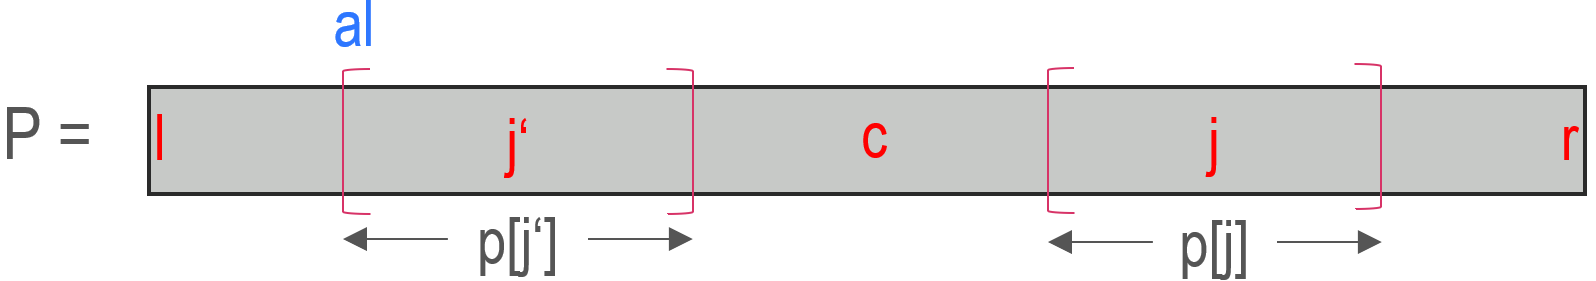
\includegraphics[width=11cm]{Bilder2/Abb2.PNG}
    \caption{Eigenschaften eines Palindromes}
    \label{fig:enter-label2}
\end{figure}

Angenommen, \textit{P} sei ein Palindrom. Die Grenzen werden durch \textit{l} und \textit{r} gekennzeichnet. Veranschaulicht durch Abbildung~\ref{fig:enter-label2} existiert ein Zeichen \textit{c}, welches das mittlere Zeichen des Palindromes \textit{P} darstellt. Bei Palindromen gerader Länge ist \textit{c} immer eine Raute. Für jedes Zeichen der rechten Teilzeichenkette des Palindromes, existiert ein identisches Zeichen innerhalb der linken Teilsequenz mit identischem Abstand zur \textit{c} und der jeweiligen Grenze. Diese zueinander korrespondierenden Zeichen müssen gleich sein, da beide innerhalb der Grenzen des Palindromes \textit{P} sich befinden. 

Der Manacher-Algorithmus bestimmt die Palindromlängen der Zeichen des Intervalls (\textit{c},\textit{r}) anhand der bekannten Palindromlängen der Zeichen des Intervalls (\textit{l},\textit{c}). In Abbildung~\ref{fig:enter-label2} wird beispielhaft die Palindromlänge des Zeichens \textit{j} gesucht. Für das identische Zeichen \textit{j'}, der linken Teilzeichenkette, ist die Palindromlänge, \textit{p[j’]}, bekannt. Die linke Grenze des inneren Palindromes von \textit{j} wird \textit{al} bezeichnet. Solange \textit{al} echt größer als \textit{l} ist, muss die rechte Grenze des inneren Palindromes von \textit{j} echt kleiner sein als \textit{r}. Sollte \textit{al}>\textit{l} gelten, muss die Palindromlängen \textit{p[j]} der Palindromlänge \textit{p[j’]} entsprechen.

Entspricht \textit{al} der linken Grenze \textit{l} oder überschreitet \textit{al} diese Grenze, muss die rechte Grenze \textit{r} erweitert werden. In diesem Fall kann \textit{p[j]} gleich oder größer als \textit{p[j’]} sein. Weitere Zeichen, nach der aktuellen rechten Grenze, könnten noch zum Palindrom \textit{p[j’]} gehören und daher kann \textit{p[j’]} größer ausfallen als \textit{p[j]}. 

Der Manacher-Algortihmus verwendet die Feld-Datenstruktur, um alle Palindromlängen zu speichern. Das Feld ist die Ausgabe des Manacher-Algorithmus. Für die minimale Sequenz, werden die maximalen Faltindizes ausgehend vom Präfix und Suffix benötigt. Die maximalen Faltindizes werden mit Präfix-Faltindex beziehungsweise Suffix-Faltindex abgekürzt. Der Präfix-Faltindex wird innerhalb eines Durchlaufs des Feldes ermittelt, aufgrund der Erkenntnisse, wie ein Präfix-Faltindex erweitert werden kann. Die präparierte Zeichenkette wird bis zum maximalen Präfix-Faltindex reduziert. Bezeichnet wird die resultierende Zeichenkette als RZ. Für RZ wird der maximale Suffix-Faltindex berechnet. Wird die resultierende Zeichenkette umgekehrt, berechnet sich der maximale Suffix-Faltindex identisch zum Präfix-Faltindex. Der  Suffix-Faltindex passt nicht zur präparierten Zeichenkette, da diese nicht umgekehrt wurde. Der Suffix-Faltindex der präparierten Zeichenkette ermittelt sich durch:
\begin{align}
(\text{Präfix-Faltindex}+\text{Größe RZ} - \text{Suffix-Faltindex der umgekehrten Zeichenkette} - 1)
\end{align}
Das Ergebnis berechnet sich aus den Faltindizes der präparierten Zeichenkette und wird durch zwei geteilt, da die präparierte Zeichenkette die Rauten enthält, welche die ursprünglichen Sequenz nicht enthielt.
\begin{align}
((\text{Suffix-Faltindex}) - (\text{Präfix-Faltindex})) / 2
\end{align}
%
\subsection{Implementierung}
\label{subsec:TextBefehle}
Die verwendeten Methoden werden im Folgenden vereinfacht dargestellt. Eine vollständige Implementierung in C++ ist im Anhang zu finden.
\begin{lstlisting}
//präpariert eine Zeichenkette
//example: input=abba; output=#a#b#b#a#
string preString(input){
    output = "#";
    //durchlaufe jedes Zeichen der ursprünglichen Zeichenkette    
    for(char c : input){
        output += c;
        output += '#';
    }    
    return output;
}
//berechnet Palindromlänge für jedes Zeichen einer Zeichenkette
vector<int> manacherAlgorithm(str){
    lengths = Ergebnisfeld
    c = Zentrum des längsten Palindromes
    r = rechte Grenze des längsten Palindromes
    //iteriert über jedes Zeichen der Eingabe
    for(int i=0; i<str.length(); i++){ 
        mirror = Position des identischen Zeichen der linken Teilzeichenkette
        //überprüft, ob sich das aktuelles Zeichen innerhalb des längsten 
        //Palindromes befindet
        if(i<r){
            lengths[i] = min(r-i, lengths[mirror]);
        }
        right = rechte Grenze des längsten Palindromes
        left = linke Grenze des längsten Palindromes
        //Palindromerweiterung des einzelnen Zeichens
        while(left>=0 && right<str.length() && str[right] == str[left]){
            lengths[i]++;
            right++;
            left--;
        }
        //falls Palindromerweiterung über right hinausgeht => Grenzen anpassen
        if(i+lengths[i]>r){
            c = i;
            r = i+lengths[i];
        }
    }
    return lengths;
}
//ermittelt den maximalen Präfix-Faltindex
int maxCut(vector<int>& lengths, string& str){
    max = 0 //Startwert
    //durchläuft alle Palindromlängen der Palindrome gerader Länge
    for(int i=2; i<=(lengths2.size()); i+=2){ 
        //überprüft, ob der Faltindex erweitert werden kann
        if((lengths2[i]>0 && lengths2[i] == i) || lengths2[i]+max >= i){
            max = i;
        }
    }
    return max;
}
\end{lstlisting}
%
\subsection{Laufzeit}
\label{subsec:TextBefehle}
Das Präparieren einer Zeichenkette benötigt einen Durchlauf aller Zeichen der ursprünglichen Zeichenkette. Der Manacher Algorithmus benötigt einen Durchlauf aller Zeichen der präparierten Zeichenkette und aktualisiert die Palindromlängen der Zeichen innerhalb konstanter Zeit. Palindromlängen einzelner Zeichen, werden direkt übernommen, falls die Grenzen des Palindromes innerhalb der bekannten Grenzen \textit{l} und \textit{r} liegen. Geht die rechte Grenze des inneren Palindromes über die rechte Grenze \textit{r} hinaus, so wird diese erweitert. Dementsprechend hat der Manacher Algorithmus eine Laufzeit von $\mathcal{O}(2N+1)$ [1], wenn \textit{N} die Eingabelänge der ursprünglichen Zeichenkette ist. Ein maximaler Präfix-Faltindex wird ebenfalls innerhalb eines Durchlauf jeder zweiten Zahl des Feldes, welches vom Manacher Algorithmus berechnet wurde, ermittelt. Jede Zahl entspricht einem Zeichen, daher benötigt die Berechnung eines maximalen Präfix-Faltindex nur einen Durchlauf der ursprünglichen Zeichenkette. Unter der Annahme, dass die ursprüngliche Sequenz aus \textit{N} Zeichen besteht, lässt sich eine asymptotische Laufzeit von $\mathcal{O}(N)$ ermitteln.
%
\subsection{Testergebnisse}
\label{subsec:TextBefehle}
Die Implementierung konnte ausschließlich anhand der gegebenen Testfälle geprüft werden. Mit Hilfe eines Python-Skripts wurden alle beispielhaften Eingaben ausgeführt. Der Anhang enthält eine Tabelle mit der Laufzeit pro Eingabe in Sekunden, zusammen mit den Resultaten. Jedes Resultat wurde mit dem erwarteten Wert verglichen. Die Resultate stimmten immer mit den erwarteten Werte überein. Außerdem benötigt keine der Eingaben für die Ausführung mehr als die vorgegebenen fünf Sekunden.
%
%
\newpage
\section{Problem I: A Safe Bet}
\label{sec:Latex}
\subsection{Beschreibung der Problemdomäne}
\label{subsec:DokHeadGli}
Ein neuer durch einen Laserstrahl gesicherter Tresor wurde erfunden. Der Tresor entspricht hier einem rechteckigen Gitter. Innerhalb des Gitters befinden sich Spiegel. Es wird zwischen zwei Arten von in einem Winkel von 45 Grad diagonal orientierten Spiegeln unterschieden. Entweder sind Spiegel von der Art “\slash” oder von der Art “\textbackslash”. 

Der Laserstrahl startet immer horizontal-links in der ersten Reihe des Tresor-Gitters. Der Tresor öffnet sich, falls der Laserstrahl horizontal-rechts aus der letzten Reihe des Tresor-Gitters austritt. Die Spiegel innerhalb des Gitters können die Richtung des Laserstrahls beeinflussen.

Nachdem der Laser eingeschaltet wurde, kann der Tresor in drei mögliche Fälle eingeordnet werden.
\begin{enumerate}
  \item Sollte sich der Tresor durch den Laserstrahl öffnen lassen, ohne dass ein weiterer Spiegel hinzugefügt wurde, gilt der Tresor als \textbf{unsicher}.
  \item Ist es nicht möglich, den Tresor nur mittels des Hinzufügens eines einzelnen Spiegels zu öffnen, gilt der Tresor als \textbf{unmöglich} zu öffnen.
  \item Sollte sich der Tresor durch das Hinzufügen genau eines Spiegels öffnen lassen, so gilt dieser als \textbf{sicher}.
\end{enumerate}
Gilt ein Tresor als sicher ist zu beachten, dass es mehr als eine Möglichkeit geben kann, den Laserstrahl nur mittels eines einzigen Spiegels zum Detektor zu lenken und somit den Tresor zu öffnen. Daher wird die Anzahl aller möglichen Spiegel, welche den Tresor öffnen könnten sowie die Koordinaten des lexikographisch kleinsten Spiegels gefordert. Der lexikographisch kleinste Spiegel wird als erstes nach der Reihe und darauf nach der Spalte des Spiegels sortiert.
%
\subsection{Erkenntnisse}
\label{subsec:TextBefehle}
Trifft der Laserstrahl auf einen Spiegel, so wechselt der Laserstrahl immer seine bisherige Ausrichtung. Die Ausrichtung des Lasers ist entweder horizontal oder vertikal. Eine Richtung, aus welcher der Laserstrahl emittiert wird, kann entweder Norden, Osten, Süden oder Westen entsprechen.
\begin{figure}[h]
    \centering
    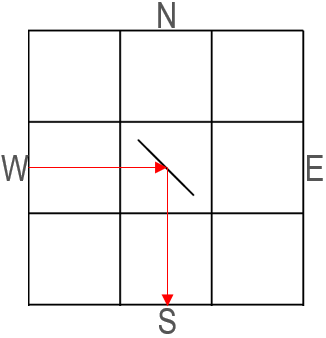
\includegraphics[width=7cm]{Bilder2/Abb3.PNG}
    \caption{Beispielhafte Spiegelung eines Laserstrahls}
    \label{fig:enter-label3}
\end{figure}

Ausgehend von dem roten Laser aus der westlichen Richtung (Abb.~\ref{fig:enter-label3}) und der Kenntnis über die Spiegelart, also “\slash” oder “\textbackslash”, kann die Ablenk-Richtung des Laserstrahls nur Süden sein. Sollte ein Laserstrahl auf einen Spiegel treffen, ist die folgende Richtung des Laserstrahls, also dessen Ablenk-Richtung, eindeutig, falls die Art des Spiegels und die Richtung, aus der der Laserstrahl emittiert worden ist, bekannt sind. 

Unterliegt der Tresor nicht dem ersten Fall, so müssen die einzelnen Spiegel bestimmt werden, welche beim Einfügen in das Tresor-Gitter den Tresor öffnen. Aus der Tresor-Beschreibung, welche Teil der erforderlichen Eingabe ist, können die Startwerte und Zielwerte des Lasers bestimmt werden. Der Start- und Endwert setzt sich aus einer \textit{x}-Koordinate und einer \textit{y}-Koordinate sowie der Richtung des Laserstrahls zusammen. Der Start des Laserstrahls ergibt sich aus den Werten (\textit{x}=1, \textit{y}=0, Osten) und der Endwert ergibt sich aus den Werten (\textit{x}=r, \textit{y}=c+1, Westen).

Anhand der Start-/Endwerte können zwei Laserstrahlen, ausgehend vom Start und ausgehend vom Ende, simuliert werden. Wenn sich die beiden Laserstrahlen schneiden, muss dies ein horizontaler Abschnitt vom Start mit einem vertikalen vom Ende oder ein vertikaler Abschnitt vom Start mit einem horizontalen vom Ende sein. Beide Laserstrahlen erreichen den Schnittpunkt, jedoch müssen ihre Ausrichtungen unterschiedlich sein. Folglich reicht ein einzelner Spiegel, damit der Laserstrahl vom Start bis zum Ende reicht. Aufgrund der Eigenschaft, dass die Spiegel die Laserstrahlausrichtung verändern, reicht genau ein Spiegel aus. 

Jeder Schnittpunkt der beiden Laserstrahlen repräsentiert einen möglichen Spiegel, welcher den Tresor öffnen würde. Sollte kein Schnittpunkt existieren, so wäre es nicht möglich, mit nur einem Spiegel den Tresor zu öffnen und der Tresor unterliegt dem zweiten Fall.
%
\subsection{Modellierung des Problems}
\label{subsec:TextBefehle}
Die in der Tresor-Beschreibung gegebenen Spiegel können innerhalb zweier Mengen gespeichert werden. Eine Menge repräsentiert alle Zeilen und speichert für jede Zeile das Vorkommen aller Spiegel innerhalb dieser. Es werden die Art des Spiegels und die zugehörige Spalte des Spiegels gespeichert. Die zweite Menge, welche alle Spalten repräsentiert, kann analog erstellt werden. Ein Laserstrahl kann durch gegebene Spiegel bezüglich seiner Richtung beeinflusst werden und besteht daher potenziell aus mehrere horizontalen und vertikalen Linien. Eine Feld-Datenstruktur speichert, wie viele horizontale Linien sich innerhalb eines Bereiches befinden.
%
\subsection{Lösungsansatz}
\label{subsec:Abb}
Eine Eingabedatei kann mehrere Tresor-Beschreibungen beinhalten. Anfangs beschreibt ein Quadrupel (\textit{r}, \textit{c}, \textit{m},\textit{n}) die Anzahl der Reihen (\textit{r}) und Spalten (\textit{c}) des Tresor-Gitters. Die nachfolgenden \textit{m}- und \textit{n}-Zeilen beschreiben die Koordinaten der "\slash”-Spiegel beziehungsweise der “\textbackslash”-Spiegel.

Anfangs werden die zwei Mengen “rows” und “columns” erstellt. Eine Menge verweist mittels Schlüssel auf Paare. In der Menge “rows” gibt es für jede Zeile einen eindeutigen Schlüssel. Der \textit{i}-te Schlüssel aus der Menge “rows” entspricht der \textit{i}-ten Zeile innerhalb des Tresor-Gitters. Die \textit{i}-te Zeile entspricht der \textit{x}-Koordinate des Spiegels. Jedes Paar der Menge “rows”, besteht aus der \textit{y}-Koordinate und der Art des jeweiligen Spiegels innerhalb der Zeile. Die \textit{y}-Koordinate entspricht der Spalte des Spiegels. Analog wird die Menge “columns” erstellt. 

Geraden innerhalb des Tresor-Gitters werden als Linien bezeichnet. Ein Laserstrahl wird durch mehrere Linien dargestellt. Eine Linie beinhaltet die Informationen “xlow”, “xhigh”, “ylow” und “yhigh”. Da Linien eindimensional sind, entspricht bei horizontalen Linien “xlow” gleich “xhigh” und bei vertikalen “ylow" gleich “yhigh”.
\begin{figure}[h]
    \centering
    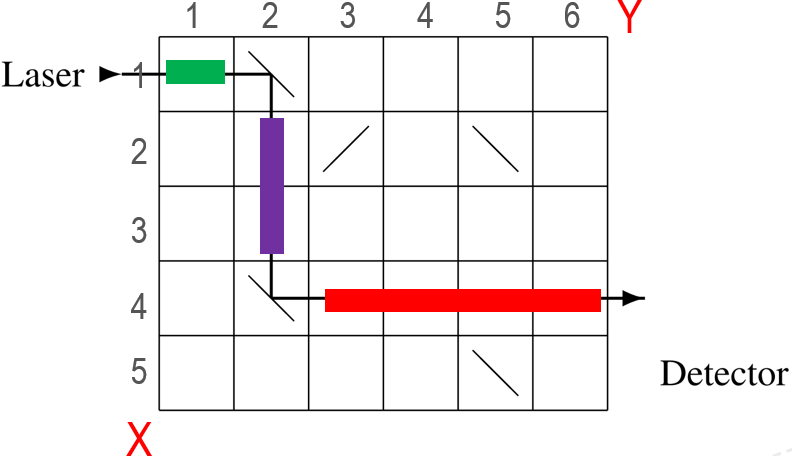
\includegraphics[width=10cm]{Bilder2/Abb4.PNG}
    \caption{Beispielhafte Linien eines Laserstrahls}
    \label{fig:enter-label4}
\end{figure}

Anhand der Abbildung~\ref{fig:enter-label4} ist zu erkennen, wie die Werte einer konkreten Linie bestimmt werden. Für die horizontale, rote Linie (Abb.~\ref{fig:enter-label4}) wären die Werte xlow=4, ylow=3, xhigh=4 und yhigh=6. Um die einzelnen Linien zu bestimmen, werden die aktuellen Koordinaten des Lasers benötigt und die aktuelle Richtung eines von dem Laser emittierten Laserstrahls. Beim Start ist der Laserstrahl aus Westen kommend ausgerichtet und die Koordinaten des Lasers sind (\textit{x}=1, \textit{y}=0). Anhand dieser Informationen kann für horizontale Linien innerhalb der “rows”-Menge nachgeschaut werden, bei welchen Koordinaten der Laserstrahl auf einen Spiegel trifft. Da die \textit{x}-Koordinate die aktuelle Zeile und somit den Schlüssel der Menge angibt, muss nur überprüft werden, wann der nächste Spiegel bezüglich der aktuellen \textit{y}-Koordinate (der Spalte) kommt. 
Für vertikale Linien wird die “columns”-Menge geprüft, ob innerhalb der aktuellen Spalte (\textit{y}-Koordinate) ein weiterer Spiegel folgt, ausgehend von der aktuellen Zeile (\textit{x}-Koordinate). Bezüglich der Richtung des Laserstrahls, kann entweder links oder rechts von der aktuellen Spalte beziehungsweise unterhalb oder oberhalb der aktuellen Zeile gesucht werden. Alle Linien werden dabei innerhalb zwei dynamischer Felder, getrennt bezüglich horizontaler und vertikaler Linien, gespeichert. Sollte es keinen Spiegel innerhalb der Zeile/Spalte mehr geben, dann ist dies die letzte Linie und der Laserstrahl endet.

Sobald der Laserstrahl, ausgehend vom Start emittiert wurde, muss überprüft werden, ob dieser bereits den Tresor öffnet. Um den Tresor zu öffnen, muss der Laserstrahl mit den Koordinaten des Detektors enden. Sollte die Koordinaten des Laserstrahls \textit{r} und \textit{c+1} entsprechen, ist der Laserstrahl am Detektor angekommen. Der Tresor wäre unsicher. Die Ausgabe für den Tresor kann direkt nach dieser Feststellung getätigt werden.

Handelt es sich jedoch um keinen unsicheren Tresor, muss ausgehend vom Ende ein weiterer Laserstrahl simuliert werden. Die Erstellung der horizontalen und vertikalen Linien ist analog, allerdings gilt es zu beachten, dass die Linien vom Start und Ende in getrennten dynamischen Feldern gespeichert werden. Daraus resultieren zwei Felder für horizontale Linien und zwei Felder für vertikale Linien.

Zum Auffinden der Schnittpunkte wird der Plane-Sweep-Algorithmus benutzt. Dieser verwendet Events, um mögliche Schnittpunkte ausfindig zu machen. Ein Event beinhaltet die Information, ob dieses zu einer vertikalen Linie gehört, einen “value”, zwei Werte ("low", "high") zur \textit{x}-Achsen Intervalleingrenzung und einen “add”-Wert. Der “value” entspricht der y-Koordinate der Linie. Anhand der \textit{y}-Koordinate werden alle Events aufsteigend sortiert. 

Zu Beginn werden alle Events erstellt. Jede horizontale Linie benötigt zwei Events. Der erste Punkt repräsentiert den Start der horizontalen Linie auf der \textit{y}-Achse. Mittels des zweiten Events wird das Ende dieser horizontalen Linie gekennzeichnet. Vertikale Linien erhalten nur ein Event, da diese nur eine \textit{y}-Koordinate beinhalten. Die Events werden aufsteigend nach ihrem “value” sortiert. Die Sortierung repräsentiert die Auslöse-Reihenfolge der Events. Falls es sich um ein horizontales Event handelt, wird immer das Feld, welches die horizontalen Linien speichert, verändert. Die Veränderung ist abhängig davon, ob es sich um den Start oder das Ende der horizontalen Linie handelt. Beim Aufruf eines vertikalen Events wird über die \textit{x}-Achse das Intervall der vertikalen Linie gebildet. Sollte im Feld, innerhalb des Intervalls, ein horizontales Event gestartet und noch nicht beendet sein, ist dies anhand der Feldeinträge erkennbar. Somit muss die vertikale Linie von einer horizontalen Linie geschnitten werden.

Die Datenstruktur des Binary Indexed Tree ermöglicht eine passende Verwaltung des Feldes. Demnach ist jeder Index des Feldes für einen Bereich von Indizes zuständig. Ein Index muss für seinen Bereich die Summe aller Einträge speichern. Der Bereich kann durch die binäre Darstellung des Index  ermittelt werden. Verändert sich ein Index, indem ein horizontales Event aufgerufen wird, können alle Indizes, welche ebenfalls ihren Summe anpassen müssen, über die Addition des “least significant bit” ermittelt werden. Für die Ermittlung einer Präfixsumme können zusätzlich zum ursprünglichen Index-Wert alle Werte der Indizes addiert werden, welche nach Subtraktion des “least significant bit” folgen. Eine Summe über ein Intervall \textit{xl} bis \textit{xr} lässt sich mittels der Subtraktion der Präfixsumme von \textit{xr} minus der Präfixsumme von \textit{xl}-1 berechnen.

Ein Index repräsentiert eine \textit{x}-Koordinate. Horizontale Linien haben nur einen \textit{x}-Wert. Der entsprechende “add” Wert des horizontalen Events wird auf den passenden Index addiert. Beim ersten horizontalen Event wird der Index (\textit{x}-Koordinate) um eins erhöht. Folglich erhöht sich die Präfixsumme innerhalb des Feldes, ab diesem Index. Die horizontale Linie hat begonnen. Beim zweiten Event wird der Index um eins erniedrigt. Ab diesem Event ist die horizontale Linie beendet. Diese wird nicht mehr in der Präfixsumme berücksichtigt und kann daher ab diesem Zeitpunkt in keinem Intervall gefunden werden. Es wird ausgeschlossen, dass nachfolgende vertikale Linien eine schon beendete horizontale Linie schneiden. Vertikale Events umfassen ein \textit{x}-Achsen-Intervall. Das Feld berechnet für das gegebene Intervall eine Summe. Sollte diese Summe größer null sein, läuft mindestens eine horizontale Linie durch das Intervall der vertikalen Linie. Diese beiden Linien bilden folglich einen Schnittpunkt. 

Nachdem die horizontalen Linien vom Start mit den vertikalen Linien vom Ende und die vertikalen Linien vom Start mit den horizontalen Linien vom Ende auf Schnittpunkte geprüft wurden, erfolgt die Ausgabe. Gibt es keinen Schnittpunkt, ist der Tresor unmöglich zu öffnen. Sollte es Schnittpunkte geben, so wird die Anzahl der Schnittpunkte aufaddiert. Direkt nachdem ein Schnittpunkte gefunden wird, welcher lexikographisch kleinere Koordinaten als der aktuell kleinste Schnittpunkt besitzt, wird dieser Schnittpunkt zum lexikographisch kleinsten. Der lexikographisch kleinste Spiegel entspricht dem lexikographisch kleinsten Schnittpunkt. Für einen sicheren Tresor kann somit die Summe aller möglichen einzelnen Spiegel und die Koordinaten des lexikographisch kleinsten Spiegels ausgegeben werden.
%
\subsection{Implementierung}
\label{subsec:TextBefehle}
Die Implementierung beinhaltet eine vereinfachte Darstellung der benötigten Klassen und Methoden. Eine vollständige Implementierung in C++ ist im Anhang zu finden.
\begin{lstlisting}
tree = Feld zum Speichern der horizontalen Events 
lowestX = x-Koordinate des lexikographisch kleinsten Schnittpunkts 
lowestY = y-Koordinate des lexikographisch kleinsten Schnittpunkts

rows = Menge der Zeilenspiegel
columns = Menge der Spaltenspiegel 

//horizontale/vertikale Linien
class line{
    public:
        //Parameter einer Linie
        int xlow, ylow, xhigh, yhigh;
}

//Events 
class event{
    public:
        //Parameter eines Events
        bool vertical;
        int value, low, high, add;

        bool operator < (const event &other)const{
            //Anordnungsrelation der Events 
        }
};

//Emittiert einen Laserstrahl
void laserbeam(hori, verti, x, y, dir){ 
    while(Laserstrahl trifft nicht den Gitterrand){
        //überprüfe die aktuelle Richtung
        if(dir == W){
            auto it = nächster Spiegel innerhalb des passenden Sets

            if(it == rows[x].begin()){
                //Laserstrahl trifft den Gitterrand
            }else{
                //Bestimmung neuer Richtung
            }
        }else if(dir == S){
            analog
        }           
        }else if(dir == E){
            analog
        }
        }else if(dir == N){
            analog
        }
        //Speichern der Linien getrennt nach horizontalen/vertikalen
        if(nextX == x){
            hori.emplace_back(line{x, min(y, nextY)+1, x, max(y, nextY)-1});
        }else if(nextY == y){
            verti.emplace_back(line{min(x, nextX)+1, y, max(x, nextX)-1, y});
        }
        //nächsten Koordinaten
        x = nextX;
        y = nextY;
    }
    //prüft, ob der Laserstrahl im Detektor endet
    if(x == r && y == c+1){
        without = true;
    }
}

void update(int pos, int value){
    addiert einen übergebenen Wert auf alle Positionen eines Binary Indexed Tree
}

big prefixSum(int pos){
    berechnet eine Präfixsumme bis zu einer gegebenen Position
}

big intervalSum(int left, int right){
    //berechnet Intervallsummen vertikaler Events
    return prefixSum(right) - prefixSum(left-1);
}

//berechnet Schnittpunkte 
big intersections(hori, verti){
    e = Liste aller Events
    //erstellt alle horizontalen und vertikalen Events
    for(auto h : hori){
        e.emplace_back(false, h.ylow, h.xlow, h.xlow, 1);
        e.emplace_back(false, h.yhigh, h.xlow, h.xlow, -1);
    }
    for(auto v : verti){
        e.emplace_back(true, v.ylow, v.xlow, v.xhigh, -1);
    }
    sort(e.begin(), e.end());
    //iteriert über alle sortierten Events
    for(auto e1 : e){
        //vertikales Event
        if(e1.vertical){
            int low = e1.low;
            int high = e1.high;
            inter = Intervallsumme der x-Koordinaten des vertikalen Events
            //entspricht die Intervallsumme mind. 1 => Schnittpunkt
            if(inter <= 0){
                continue;
            }
            while(low < high){
                int mid = (low + high)/2;
                //Binäre Suche der exakten Koordinaten des Schnittpunkts
            }
            //Vergleich des Schnittpunkts mit dem aktuell lexikographisch 
            //kleinsten Schnittpunkts
                     
            result = Speichert die Anzahl der gefundenen Schnittpunkte

        //horizontales Event
        }else{
            //Feldveränderung
        }
    }
    return result;
}   
\end{lstlisting}
%
\subsection{Laufzeit}
\label{subsec:TextBefehle}
Die Sets “rows” und “columns” speichern Spiegelinformationen. Dazu wird pro Set jeder Spiegel einmalig benötigt. Es gibt (\textit{m}+\textit{n})-viele Spiegel, folglich unterliegt die Initialisierung der Sets einer konstanten Laufzeit von $\mathcal{O}(m+n)$, da \textit{m} und \textit{n} bekannte Konstanten sind. Innerhalb des Tresor-Gitters kann es bis zu \textit{rc} Linien geben, welche einem Laserstrahl zugeordnet werden. Somit kann es bis zu $\mathcal{O}(rc)$ Zeit benötigen, um einen Laserstrahl zu emittieren. Ausgehend von \textit{e}-vielen Events für eine Tresor-Beschreibung, benötigt der Plane-Sweep-Algorithmus für das Ausführen der "\text{update}"\text{-Funktion} $\mathcal{O}(elog(e))$ und für die Berechnung einer Intervallsumme ebenfalls $\mathcal{O}(elog(e))$ [2]. Folglich werden alle Schnittpunkte innerhalb einer Laufzeit von $\mathcal{O}(elog(e))$ berechnet. Zusammengefasst ergibt sich eine asymptotische Laufzeit pro Tresor-Beschreibung von $\mathcal{O}(rc+elog(e))$. 
\subsection{Testergebnisse}
\label{subsec:TextBefehle}
Die Implementierung wurde erfolgreich mittels des Online-Judge-Tools getestet. Darüber hinaus wurden alle bereitgestellten Testfälle mithilfe eines Python-Skripts ausgeführt. Die Laufzeit pro Testfall in Sekunden ist in einer Tabelle im Anhang aufgeführt. Zur Bestätigung ist ein Screenshot der Ergebnisse aus dem Online-Judge beigefügt.
%
%
\newpage
\appendix
\section{Anhang}
\label{sec:Latex}
\subsection{Vollständige Implementierung Gene Folding}
\label{subsec:DokHeadGli}
\begin{minted}{c++}
#include <iostream>
#include <vector>
#include <algorithm>

using namespace std;

//prepossessing of a string to compute the length of even palindromes
string preString(string& str){
    string preStr = "#";    
    for(char c : str){
        preStr += c;
        preStr += '#';
    }    
    return preStr;
}

//computes the palindrome length for each char as center of the palindrome
vector<int> manacherAlgorithm(string& str){
    vector<int> lengths(str.length(),0);
    int c=0, r=0;
    for(int i=0; i<str.length(); i++){
        int mirror = 2*c-i;
        if(i<r){
            lengths[i] = min(r-i, lengths[mirror]);
        }
        int right = i+(1+lengths[i]);
        int left = i-(1+lengths[i]);
        while(left>=0 && right<str.length() && str[right] == str[left]){
            lengths[i]++;
            right++;
            left--;
        }
        if(i+lengths[i]>r){
            c = i;
            r = i+lengths[i];
        }
    }
    return lengths;
}

//computes the maximum prefix-palindrome index
int maxCut(vector<int>& lengths, string& str){
    int max=0;
    vector<int> lengths2 = lengths;
    for(int i=2; i<=(lengths2.size()); i+=2){
        if((lengths2[i]>0 && lengths2[i] == i) || lengths2[i]+max >= i){
            max = i;
        }
    }
    return max;
}

int main()
{   
    string input;
    cin >> input;
    
    //prefix
    string preStr = preString(input);
    vector<int> result = manacherAlgorithm(preStr);
    int prefixMax = maxCut(result, input);

    //suffix
    preStr = preStr.substr(prefixMax, preStr.length());
    vector<int> result2 = manacherAlgorithm(preStr);
    reverse(result2.begin(), result2.end());
    input = input.substr(prefixMax/2,input.length()-1);
    int suffixMax = prefixMax + result2.size()-maxCut(result2, input)-1;

    //computes the chars of the remaining string
    int res = ((suffixMax)-(prefixMax))/2;
    cout << res << endl;
    return 0;
}
\end{minted}
%
\subsection{Testskript Gene Folding}
\label{subsec:TextBefehle}
\begin{minted}{python}
import os
import subprocess
import time

cpp_program = "C:\\Users\\morit\\effiziente-algorithmen\\Gene Folding\\mainfinal.exe"
input_folder = "C:\\Users\\morit\\Desktop\\D-genefolding"
output_folder = "C:\\Users\\morit\\Desktop\\Laufzeit_GeneFolding"
output_file = "C:\\Users\\morit\\Desktop\\runtimes.txt"

with open(output_file, "w") as runtime_file:
    for filename in os.listdir(input_folder):
        if filename.endswith(".in"):
            input_path = os.path.join(input_folder, filename)
            ans_path = os.path.join(input_folder, filename.replace(".in", ".ans"))

            with open(input_path, "r") as file:
                input_string = file.read()

            start_time_case = time.time()

            result = 
            subprocess.run([cpp_program], input=input_string.encode(), 
            text=False, capture_output=True)

            end_time_case = time.time()
            duration_case = end_time_case - start_time_case

            input_length = len(input_string)

            cpp_output = result.stdout.decode()

            with open(ans_path, "r") as out_file:
                expected_output = out_file.read()

            is_correct = cpp_output.strip() == expected_output.strip()

            runtime_file.write(f"File: {filename}\n")
            runtime_file.write(f"Input Length: {input_length}\n")
            runtime_file.write(f"Result: {cpp_output}\n")
            runtime_file.write(f"Expected: {expected_output}\n")
            runtime_file.write(f"Correct: {is_correct}\n")
            runtime_file.write(f"Duration: {duration_case} seconds\n\n")

\end{minted}
%
\subsection{Testergebnisse Gene Folding}
\label{subsec:Mathematik}
\afterpage{%NEUE
\centering%NEUE
\begin{tabular}[h]{c|c|c|c|c|c}
     \textbf{Inputfile} & \textbf{Duration (s)} & \textbf{Correct?} & \textbf{Inputfile} & \textbf{Duration (s)} & \textbf{Correct?} \\
     \hline
     sample-1.in & 0.06543 & yes & sample-2.in & 0.01583 & yes \\
     secret-001.in & 0.11616 & yes & secret-002.in & 0.62825 & yes \\
     secret-003.in & 0.01526 & yes & secret-004.in & 0.02655 & yes \\
     secret-005.in & 0.01907 & yes & secret-006.in & 0.01897 & yes \\
     secret-007.in & 0.01834 & yes & secret-008.in & 0.01410 & yes \\
     secret-009.in & 0.01492 & yes & secret-010.in & 0.75532 & yes \\
     secret-011.in & 0.60981 & yes & secret-012.in & 0.62144 & yes \\
     secret-013.in & 0.55981 & yes & secret-014.in & 0.64379 & yes \\
     secret-015.in & 0.76912 & yes & secret-016.in & 0.75671 & yes \\
     secret-017.in & 0.75874 & yes & secret-018.in & 0.71544 & yes \\
     secret-019.in & 0.01570 & yes & secret-020.in & 0.01893 & yes \\
     secret-021.in & 0.01506 & yes & secret-022.in & 0.02276 & yes \\
     secret-023.in & 0.01576 & yes & secret-024.in & 0.01559 & yes \\
     secret-025.in & 0.01548 & yes & secret-026.in & 0.01602 & yes \\
     secret-027.in & 0.01517 & yes & secret-028.in & 0.02377 & yes \\
     secret-029.in & 0.02564 & yes & secret-030.in & 0.02036 & yes \\
     secret-031.in & 0.02834 & yes & secret-032.in & 0.02609 & yes \\
     secret-033.in & 0.01941 & yes & secret-034.in & 0.02104 & yes \\
     secret-035.in & 0.01787 & yes & secret-036.in & 0.03192 & yes \\
     secret-037.in & 0.02149 & yes & secret-038.in & 0.02726 & yes \\
     secret-039.in & 0.01929 & yes & secret-040.in & 0.02921 & yes \\
     secret-041.in & 0.02690 & yes & secret-042.in & 0.03223 & yes \\
     secret-043.in & 0.02542 & yes & secret-044.in & 0.04140 & yes \\
     secret-045.in & 0.02114 & yes & secret-046.in & 0.02085 & yes \\
     secret-047.in & 0.02565 & yes & secret-048.in & 0.03940 & yes \\
     secret-049.in & 0.02083 & yes & secret-050.in & 0.01802 & yes \\
     secret-051.in & 0.02347 & yes & secret-052.in & 0.02402 & yes \\
     secret-053.in & 0.01463 & yes & secret-054.in & 0.02247 & yes \\
     secret-055.in & 0.01695 & yes & secret-056.in & 0.02846 & yes \\
     secret-057.in & 0.02556 & yes & secret-058.in & 0.02624 & yes \\
     secret-059.in & 0.02466 & yes & secret-060.in & 0.02533 & yes \\
     secret-061.in & 0.02245 & yes & secret-062.in & 0.02739 & yes \\
     secret-063.in & 0.02937 & yes & secret-064.in & 0.01963 & yes \\
     secret-065.in & 0.85391 & yes & secret-066.in & 0.51321 & yes \\
     secret-067.in & 0.48282 & yes & secret-068.in & 0.48664 & yes \\
     secret-069.in & 0.50982 & yes & secret-070.in & 0.57523 & yes \\
     secret-071.in & 0.58711 & yes & secret-072.in & 0.67772 & yes \\
     secret-073.in & 0.49654 & yes & secret-074.in & 0.59495 & yes \\
     secret-075.in & 0.59470 & yes & secret-076.in & 0.51979 & yes \\
     secret-077.in & 0.59301 & yes & secret-078.in & 0.64789 & yes \\
     secret-079.in & 0.52325 & yes \\
\end{tabular}
\clearpage%NEUE
}
%
\subsection{Vollständige Implementierung A Safe Bet}
\label{subsec:DokHeadGli}
\begin{minted}{c++}
#include <iostream>
#include <vector>
#include <algorithm>
#include <stdio.h>
#include <set>
#include <string.h>

using namespace std;

//possible directions for the laser beam
#define N 0
#define E 1
#define S 2
#define W 3
#define MAX 2000000

int r, c, tree[MAX], lowestX = 1000000000, lowestY = 1000000000;
bool without;
typedef pair<int,int> p;
typedef long long int big;

set<p> rows[MAX];
set<p> columns[MAX];

//line objects for horizontal and vertical laser sections
class line{
    public:
        //start and end points of straight lines
        int xlow, ylow, xhigh, yhigh;
    
        line(int xl, int yl, int xh, int yh) : xlow(xl), ylow(yl), xhigh(xh), yhigh(yh){} 
};

//events for plane-sweep
class event{
    public:
        bool vertical;
        int value, low, high, add;

        event(bool ver, int val, int l, int h, int a) : vertical(ver), value(val), low(l),
        high(h), add(a){}

        bool operator < (const event &other)const{
            if(value != other.value){
                return value < other.value;
            }else if(add != other.add){
                return add > other.add;
            }else{
                return vertical > other.vertical;
            }
        }
};

//simulation of a laser beam as lines
void laserbeam(vector<line> &hori, vector<line> &verti, int x, int y, int dir){ 
    int nextX, nextY;
    bool next = true;

    while(next){
        //West
        if(dir == W){
            nextX = x;   
            nextY = 0;   //default
            auto it = rows[x].lower_bound({y,-1});

            if(it == rows[x].begin()){
                next = false;
            }else{
                it--;
                nextY = it->first;
                //next direction
                if(it->second){
                    dir = N;
                }else{
                    dir = S;
                }
            }
        //South 
        }else if(dir == S){
            nextX = r+1;   //default
            nextY = y;   
            auto it = columns[y].upper_bound({x,1000000000});

            if(it == columns[y].end()){
                next = false;
            }else{
                nextX = it->first;
                //next direction
                if(it->second){
                    dir = E;
                }else{
                    dir = W;
                }
            }
        //East           
        }else if(dir == E){
            nextX = x;   
            nextY = c+1;   //default
            auto it = rows[x].upper_bound({y,1000000000});

            if(it == rows[x].end()){
                next = false;
            }else{
                nextY = it->first;
                //next direction
                if(it->second){
                    dir = S;
                }else{
                    dir = N;
                }
            }
        //North
        }else if(dir == N){
            nextX = 0;   //default
            nextY = y;   
            auto it = columns[y].lower_bound({x,-1});

            if(it == columns[y].begin()){
                next = false;
            }else{
                it--;
                nextX = it->first;
                //next direction
                if(it->second){
                    dir = W;
                }else{
                    dir = E;
                }
            }            
        }

        if(nextX == x){
            hori.emplace_back(line{x, min(y, nextY)+1, x, max(y, nextY)-1});
        }else if(nextY == y){
            verti.emplace_back(line{min(x, nextX)+1, y, max(x, nextX)-1, y});
        }
        x = nextX;
        y = nextY;
    }
    //ends the laser in the detector
    if(x == r && y == c+1){
        without = true;
    }
}

//adds the value (= "add") to the given position and all subsequent positions (in the tree)
void update(int pos, int value){
    if(pos <= 0){
        return;
    }
    for(pos; pos < MAX; pos += (pos & -pos)){
        tree[pos] += value;
    }
}

//computes the prefix sum for a given position (from the tree)
big prefixSum(int pos){
    big result = 0;
    if(pos <= 0){
        return 0;
    }
    for(pos; pos>0; pos -= (pos & -pos)){
        result += tree[pos];
    }
    return result;
}

//computes the number of horizontal lines which cross the given section
big intervalSum(int left, int right){
    if(left>right){
        return 0;
    }
    return prefixSum(right) - prefixSum(left-1);
}

//computes all intersections for horizontal and vertical lines and stores the 
//lexicographically smallest
big intersections(vector<line> hori, vector<line> verti){
    memset(tree,0,sizeof tree);
    vector<event> e;
    big result = 0;

    //generate all events
    for(auto h : hori){
        e.emplace_back(false, h.ylow, h.xlow, h.xlow, 1);
        e.emplace_back(false, h.yhigh, h.xlow, h.xlow, -1);
    }
    for(auto v : verti){
        e.emplace_back(true, v.ylow, v.xlow, v.xhigh, -1);
    }
    sort(e.begin(), e.end());

    for(auto e1 : e){
        //vertical line
        if(e1.vertical){
            int low = e1.low;
            int high = e1.high;
            big inter = intervalSum(low, high);
            if(inter <= 0){
                continue;
            }
            //binary search to find precise intersection
            while(low < high){
                int mid = (low + high)/2;
                if(intervalSum(e1.low, mid) >= 1){
                    high = mid;
                }else{
                    low = mid+1;
                }
            }
            //keep track of the lexicographically smallest mirror
            if(low < lowestX){
                lowestX = low;
                lowestY = e1.value;
            }else if(low == lowestX && e1.value < lowestY){
                lowestY = e1.value;
            }            
            result += inter;

        //horizontal line
        }else{
            update(e1.low, e1.add);
        }
    }
    return result;
}

int main()
{   
    int curCase = 0;
    int m, n, x, y;

    while(scanf("%d%d%d%d", &r, &c, &m, &n) > 0){
        curCase++;

        //empty the sets rows and columns
        for(int i=0; i<=r+1; i++){
            rows[i].clear();
        }
        for(int i=0; i<=c+1; i++) {
            columns[i].clear();
        }

        //fill the rows and colums sets with "/"-mirrors (represented by 0)
        for(int i=0; i<m; i++){
            scanf("%d%d", &x, &y);
            rows[x].insert({y, 0});
            columns[y].insert({x, 0});
        }

        //fill the rows and colums sets with "\"-mirrors (represented by 1)
        for(int i=0; i<n; i++){
            scanf("%d%d", &x, &y);
            rows[x].insert({y, 1});
            columns[y].insert({x, 1});
        }

        //resets
        lowestX = 1000000, lowestY = 1000000;
        without = false;

        //laser starting at the top left of the grid (start point)
        vector<line> horiStart;
        vector<line> vertiStart;
        laserbeam(horiStart, vertiStart, 1, 0, E);

        //safe opens without inserting a mirror
        if(without){
            cout << "Case " << curCase << ": 0\n";
            continue;
        }

        //laser starting at the bottom right of the grid (end point)
        vector<line> horiEnd;
        vector<line> vertiEnd;
        laserbeam(horiEnd, vertiEnd, r, c+1, W);

        //count intersections
        big num = 0;
        num += intersections(horiStart, vertiEnd);
        num += intersections(horiEnd, vertiStart);

        //output
        if(num == 0){
            cout << "Case " << curCase << ": impossible\n";
        }else{
            cout << "Case " << curCase << ": " << num << " " << lowestX 
            << " " << lowestY << '\n';
        }
    }
    return 0;
}    
\end{minted}
%
\subsection{Testskript A Safe Bet}
\label{subsec:TextBefehle}
\begin{minted}{python}
import os
import subprocess
import time

cpp_program = "C:\\Users\\morit\\effiziente-algorithmen\\1287 A Safe Bet\\works.exe"
input_folder = "C:\\Users\\morit\\Desktop\\safe"
output_file = "C:\\Users\\morit\\Desktop\\runtimesSafe.txt"

with open(output_file, "w") as runtime_file:
    runtime_file.write("\\begin{longtable}{|l|l|}\n")
    runtime_file.write("\\hline\n")
    runtime_file.write("\\textbf{File} & \\textbf{Duration (s)} \\\\\n")
    runtime_file.write("\\hline\n")
    for filename in os.listdir(input_folder):
        if filename.endswith(".in"):
            input_path = os.path.join(input_folder, filename)

            with open(input_path, "r") as file:
                input_string = file.read()

            start_time_case = time.time()

            result = subprocess.run([cpp_program], input=input_string.encode(), text=False,
            capture_output=True)

            end_time_case = time.time()
            duration_case = end_time_case - start_time_case  # Sekunden

            runtime_file.write(f"{filename} & Duration: {duration_case:.4f} \\\\\n")
            runtime_file.write("\\hline\n")
    runtime_file.write("\\end{longtable}\n")    
\end{minted}
%
\subsection{Testergebnisse A Safe Bet}
\label{subsec:Mathematik}
\centering
\begin{tabular}[h]{c|c}
    \textbf{Inputfile} & \textbf{Duration (s)} \\
    \hline
    safe-001.in & Duration: 0.6788 \\
    safe-002.in & Duration: 0.2574 \\
    safe-003.in & Duration: 0.1923 \\
    safe-004.in & Duration: 0.1627 \\
    safe-005.in & Duration: 0.1697 \\
    safe-006.in & Duration: 0.2852 \\
    safe-007.in & Duration: 0.1860 \\
    safe-008.in & Duration: 0.1586 \\
    safe-009.in & Duration: 0.2234 \\
    safe-010.in & Duration: 0.2942 \\
    safe-011.in & Duration: 0.1864 \\
    safe-012.in & Duration: 0.2163 \\
    safe-013.in & Duration: 0.1959 \\
    safe-014.in & Duration: 0.1851 \\
    safe-015.in & Duration: 0.2584 \\
    safe-016.in & Duration: 1.1117 \\
    safe-017.in & Duration: 0.1507 \\
\end{tabular}
\begin{figure}[h]
    \centering
    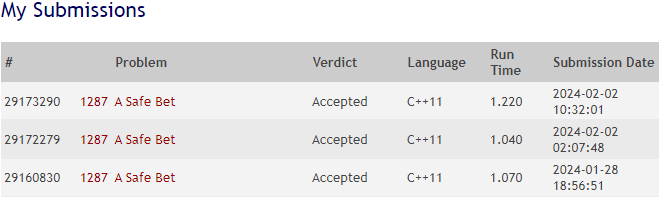
\includegraphics[width=14cm]{Bilder2/Abb6.PNG}
    \caption{Online-Judge Ausgabe.}
    \label{fig:enter-label}
\end{figure}
%
\begin{thebibliography}{99}
    \bibitem{bib:baeldung} Said Sryheni, Palindromic Substrings in O(N) with Manacher's Algorithm, \url{https://www.baeldung.com/cs/manachers-algorithm}, 8. Juni 2023.
    \bibitem{bib:boehm} Christian Böhm, Kapitel 6: Algorithmen der Computer-Geometrie, \url{https://www.dbs.ifi.lmu.de/Lehre/GIS/WS1112/Skript/GIS_WS11_06.pdf}, 2009.
    % Weitere Einträge
\end{thebibliography}
%
%
%\input{Anhang} % Der Anhang ist in einer externen Datei "Anhang.tex" und wird hier in das Dokument eingefügt.

%\printbibliography[]
\vfill
\newpage
\section*{Erklärung}
Hiermit versichere ich, dass ich diese Arbeit selbstständig verfasst und keine anderen als die angegebenen Quellen und Hilfsmittel verwendet habe.
\begin{tabular}{@{}p{2.5in}p{2.5in}@{}}
 \\[5\bigskipamount]
  \dotfill & \dotfill \\
  Student & Date
  \centering
  
\end{tabular}

\end{document}
